\documentclass[12pt,a4paper,titlepage]{article}
\usepackage[utf8]{inputenc}
\usepackage{csquotes}
\usepackage[T1]{fontenc}
\usepackage{amsmath}
\usepackage{amsfonts}
\usepackage{amssymb}
\usepackage[left=3cm,right=3cm,top=2.5cm,bottom=2.5cm]{geometry}
\usepackage{hyperref}
\usepackage[czech]{babel}
\usepackage[
  backend=biber,
  style=iso-numeric,
  maxbibnames=99
]{biblatex}
\addbibresource{maturitni_prace.bib}
\usepackage{graphicx}
\usepackage{minted}
\usepackage{subcaption} %  for subfigures environments 
%% Some packages you will need
\usepackage{tikz}
\usepackage{pgfplots}
\graphicspath{ {./images/} }

\usepackage{setspace}
\fontfamily{ptm}
\usepackage{tabularx,ragged2e,booktabs}

\DeclareBibliographyCategory{skipbibliography}
\DeclareCiteCommand{\fcite}[\mkbibfootnote]
  {\usebibmacro{prenote}}
  {\addtocategory{skipbibliography}{\thefield{entrykey}}%
   \usedriver
     {\DeclareNameAlias{sortname}{default}}
     {\thefield{entrytype}}}
  {\multicitedelim}
  {\usebibmacro{postnote}}

\author{Antonín Vřešťál}
\title{Tvorba astronomických videí}
\renewcommand{\baselinestretch}{1.5} 


\begin{document}
\maketitle

\tableofcontents
\newpage
Prohlášení a poděkování přijde sem
\newpage
\part{Teoretická část}
\section{Úvod}
\section{Postup vytváření videa} \label{makingof}
\subsection{Výběr téma a shromažďování podkladů (WIP)}
Výběr témat začíná vždy konverzací mezi jednotlivými členy. Faktory které řešíme jsou aktuální události, možnost jednotlivých členů pracovat a nálada v celém kolektivu ohledně daného téma. Následně se společně dohodneme na věcech, které bychom rádi v případném videu na dané téma probrali. (zde i v další části přijde část s Danem [naším editorem] a Terkou [naší dabérkou], kterou ještě nemám)
\subsection{Příprava textových a zvukových podkladů}
\subsection{Animování oblohy v programu Stellárium} \label{makingof:stellarium}
Celý proces začíná se scénářem. Ze scénáře si vypíši seznam přechodů a jednotlivých scén. Pro tento úkol jsem si vytvořil speciální formát zápisu, který zachytává vše, co budu potřebovat k vytvoření každého přechodu ve videu. Viz tabulka \ref{tab:scenar}.
Většina animací, které se v těchto videích nachází, byly vytvořeny pomocí simulačního programu Stellarium. Tento program je open-source (jeho zdrojový kód je volně dostupný) a jeho oficiálním účelem je realistická simulace noční oblohy při pohledu očima nebo dalekohledem\fcite{stellarium:homepage}. Stellarium poskytuje širokou nabídku programovatelných rozhraní, ať už webový server, přes který lze instanci Stellaria ovládat z prohlížeče nebo skriptovací rozhraní, které umožňuje interakci s většinou částí Stellaria pomocí programovacího jazyka, založeného na standardu ECMAScript, využívaného například jazykem JavaScript nebo ActionScript\fcite{wiki:ecmascript}.

Největším problémem pro využití Stellaria v produkci videí je fakt, že Stellarium není pro tento úkol stavěno. Neexistuje žádná funkce, která by Stellariu řekla \enquote{Otoč se plynule na tyto souřadnice a při tom vytvoř video}. Jediná možnost tvorby videa je export každého snímku finálního jako separátní soubor a tyto jednotlivé soubory poté spojit pomocí nástroje jako FFmpeg. Zde ale vznikne další problém. Tyto jednotlivé snímky musí být rovnoměrně rozloženy po celé trajektorii přechodu. Tento problém je jeden z nejobvyklejších problémů a také důvod, proč jsem přešel od manuálních animací k plně automatizovaným skriptům. Tento problém se nejčastěji řeší pomocí lineární interpolace. Základní rovnici této transformace můžete vidět níže.
\[c = (1-t)*a + t * b\] 
Kde $t$ představuje faktor v intervalu $\langle0;1\rangle$, který postupně interpoluje mezi hodnotami $a$ a $b$. Tento přechod je těžko vizualizovatelný v papírové podobě a je tedy dostupný na \url{https://c.itoncek.space/maturitni_prace/lerp_1}. Tato demonstrace ukazuje hlavní nevýhodu tohoto přístupu. Animace je sice plynulá, ale začátky a konce jsou značně trhané. Ve finálních animacích tedy používáme ještě jeden mezikrok, který vytvoří novou proměnnou $u$ pomocí následující rovnice:
\[u = (1 - t) * t^2 + t * (1-(1-x)^2))\]
Tato rovnice by se v kódu dala zjednodušit na kód, který provede lineární interpolaci podle $t$, kde hodnota $a$ bude $t^{2}$ a hodnota $b$ bude $1-(1-t)^{2}$. Tento přechod se často označuje \textit{easeInOutQuad} a jeho hlavní výhodou je jeho relativní plynulost. Průběh a rychlost lineárního a kvadratického přechodu je porovnána na grafech \ref{graph:lerp_linear} a \ref{graph:lerp_quadr}; vizuální reprezentace je dostupná na \url{https://c.itoncek.space/maturitni_prace/lerp_2}. Častými náhradami Kvadratického přechodu jsou Kubické a Kvartické ekvivalenty, které začínají sice plynuleji, ale během cesty naberou výrazně vyšší rychlost, která může být potenciálně nepříjemná pro diváky. Další nevýhodou je relativní složitost vyjádření Kubického a Kvartického přechodu pomocí jednotlivé funkce. Tyto přechody jsou často simulovány spojením dvou identických funkcí v $t=\frac{1}{2}$. Pro náš projekt jsem z těchto důvodů zvolil Kvadratický přechod.

StellariumPanoramaCreator, jak se nazývá nástroj, který jsem pro tento úkol vytvořil, plní úlohu generátoru skriptů. Tento nástroj je volně dostupný na adrese \url{https://github.com/IToncek/StellariumPanoramaCreator}. Při svém běhu postupně prochází skrze předprogramované instrukce, které jsou zabudované přímo ve zdrojovém kódu a generuje podle nich řádky skriptu a případné složky, potřebné pro úspěšný běh skriptu. Mezi funkcemi, které jsou často využívány se nachází například \textit{setup()}, která připraví Stellarium pro zaznamenávání videí (vypne veškerá překrytí, změní model atmosféry, skryje objekty Sluneční soustavy, ...), \textit{move()}, která otočí kameru na pozici, dodanou v parametru \textit{orientation} a nastaví datum a čas, dodaný v parametru \textit{datetime}. Další funkcí, která je často využívaná je funkce \textit{cheese()}, která pořídí snímek v aktuální orientaci a uloží ho ve formátu TIFF se specifickým jménem.

Z těchto základních funkcí jsou poté sestaveny funkce komplexnějšího rázu, jako například funkce \textit{slideTo()}, která je využívána k samotné tvorbě videa. Tato funkce vytváří naivním způsobem skriptové soubory, které pro každý snímek otočí pohled, změní čas a den, změní přiblížení a uloží pohled do souboru. Během přípravy této maturitní práce do sady funkcí přibyla nová kategorie funkcí, které nechávají veškeré výpočty Stellariu. Základní logikou je nevytvářet obrovské skripty ale nechat Stellarium vypočítat přechody interně. Toto umožňuje několik zjednodušení, jako například přechody mezi dvěma objekty bez nutnosti zadávání jejich nebeských souřadnic. Jednou z těchto nových funkcí je funkce \textit{travelTrack()}, která vytvoří plynulý přechod mezi souřadnicemi dvou objektů, nebo funkce \textit{slideTrack()}, která sleduje jeden vybraný objekt a zajistí, že na každém snímku je přesně veprostřed.

Pro ukládání využívám formát TIFF, který mi poskytuje vysoce kvalitní data, která jsou komprimována pouze bezztrátově pomocí algoritmu LZW. Jeden takový snímek má rozlišení 3840 na 2160 pixelů a velikost mezi pěti až sedmi megabajty. Dohromady má jeden přechod na disku velikost přibližně 7GB. Pro celé video by toto znamenalo velikost přes 200GB, což nejsem schopen uložit na dostatečně rychlém disku pro střih. Proto v posledním kroku příprav převedu každý přechod do formátu ProRes, který mi umožňuje tuto velikost snížit na pouhých 10GB, i za cenu malé ztráty na kvalitě. Při kompilaci jednotlivých snímků do videí také nastavím finální snímkovací frekvenci projektu, jíž je pro AstroCrew 50 sn./s.
\subsection{Kompletace videa v programu DaVinci Resolve} \label{makingof:resolve}
\subsubsection{Spojování jednotlivých částí} \label{makingof:resolve:merging}
Poté co je nahrán zvuk a vytvořeny veškeré animace následuje finální kompletace všech složek do finálního videa. Zde se poprvé potkává hlasová a obrazová složka. Na začátku každého videa máme několik videí, zatím co uvádíme obsah videa. Tato videa jsou s vesmírnou tématikou a častým kandidátem jsou záběry z mezinárodní vesmírné stanice, jelikož podléhají minimálním autorským právům. Po úvodním slovu a upozornění ohledně pravdivosti informací ve videu v závislosti na pozici pozorovatele na zemi přijde hlavní část videa. Zde se začínají přes sebe překrývat soubory vytvořené v sekci \ref{makingof:stellarium}. 

První scéna začíná bez jakýchkoliv souhvězdích viditelných a postupně jak video pokračuje, objevují se postupně další souhvězdí. Následující scény se drží velice podobné struktury, která je vidět na obrázku \ref{img:timeline}. Na začátku, a ve speciálních případech i uprostřed scény, se vyskytují animace, které jsou na snímku označeny číslem 1. V průběhu scény je jako podklad využit statický snímek, vygenerovaný v sekci \ref{makingof:stellarium}. Tento snímek je označený číslem 2 a slouží jako základ každé scény, přes který jsou poté překryty snímky souhvěždí (3) a objektů hlubokého vesmíru (5). Pro větší názornost využíváme tzv. pointer (4), animovaný klip pulzijícího čtverce se zaoblenými rohy, jež zvýrazňuje část obrazu o kterém právě pojednává scénář, jehož vizuální reprezentace je vidět jako obrázek \ref{img:pointer} . Někdy je třeba zvýraznit zvolený objekt hlubokého vesmíru na úkor pozadí, které zrovna v daném momentě není důležité. V tomto snímku je tento tzv. Adjustment Clip vidět pod číslem 6. Zvuková část se po většinu času skládá ze dvou stop: hlasové stopy (7) a hudební stopy (8). Hlasová stopa se nachází primárně mimo animace, kdy její dominantní místo nahradí hudba, která je po dobu přechodů zesílena.

Nad scénou se nachází pět až šest stop s titulky. Tyto stopy využíváme nejen pro standardní využití ve formě titulků v Češtině a někdy i v Angličtině, ale využíváme je i jako prostor pro citování zdrojů obrazových materiálů, opravě chyb v již vydaném videu, poznámky a doplnění obsahu od editora a stopa s informacemi a zdrojích hudby. Tento postup využíváme hlavně kvůli jednoduchosti tvorby titulků a možnosti tyto titulky skrýt a nebýt jimi rušen. 

Souhvězdí a objekty hlubokého vesmíru jsou řazeny podle nejlepšího času pozorování od západu slunce k východu slunce. Poté nastává část, kde zmíníme nejdůležitější události, které v průběhu měsíce nastávají. Na tomto místě zmiňujeme meteorické roje a atmosférické i vesmírné úkazy, které se mohou v průběhu měsíce ukázat.
\subsubsection{Mixování obrazové části}
Záběry jsou vrstveny přes sebe pomocí metody Lighten. Tato metoda pro každý pixel vypočítá barvu podle rovnice $[\max(r_1, r_2), \max(g_1, g_2), \max(b_1, b_2)]$,\fcite{wiki:blend} kde tato množina představuje červený, zelený a modrý kanál v tomto pořadí. Toto umožňuje světlým obrázkům souhvězdí překrývat se, aniž by bylo třeba odstraňovat u každého pozadí. Tento způsob mixování také využívám pro fotografie objektů hlubokého vesmíru. 

Nejdříve získám obrázek daného objektu z internetu. Nejčastějším zdrojem je Wikipedie, která poskytuje jasné licenční podmínky. Pokud na Wikipedie nemá vhodný nebo dostatečně kvalitní obrázek, začnu hledat po internetu další fotografie. Občas ani tento krok nepomůže, zvláště u objektů nezajímavých pro focení. V tomto případě se otočím na celooblohové sady dat, například Digitized Sky Survey 2 nebo Mellinger color optical survey které získávám z Centra astronomických dat univerzity ve Štrasburku díky jejich nástroji Aladin. Tyto sady dat pokrývají značný zlomek celé oblohy a z geografické pozice České republiky pokrývají 100\% viditelné oblohy. Tyto fotografie následně upravuji pomocí software Zoner Photo Studio X, kde upravím kontrast pozadí tak, aby bylo absolutně černé a tudíž při kompletaci zmizelo. Následně odstraním hvězdy blízko okraje snímku, aby byl přechod mezi snímkem a pozadím méně znatelný. Tyto fotografie jsou následně překrývány přes souhvězdí a pozadí. 
\subsection{Mixování zvukové části}
Ve zvukové části jsou na sebe navrstveny stopy hudby a hlasu. Hudbu jsem vlastnoručně vybíral ze seznamu hudby v knihovně YouTube a ze seznamu skladeb, využívaných softwarem SpaceEngine. Základním kritériem je, aby hudba nijak diváka nerušila ale zároveň pomáhala s atmosférou celého videa. Jako úvodní hudbu v našich videích používáme stopu \textit{Beyond - Patrick Patrikios} ze zvukové knihovny YouTube. V hlavní části se objevují stopy z software SpaceEngine, jako například \textit{Space G Lydian - Alfred Potter}, \textit{The Blithering Heights - Akira} a \textit{A peaceful Place - Goodstreet}. Jako naší koncovou hudbu využíváme stopu \textit{Instant Crush - Corbyn Kites} znovu ze Zvukové knihovny YouTube.
\section{Historie popularizace astronomie (WIP)}
Test \fcite{arxiv:astronomy_society}
\section{Historie a vývoj procesu tvorby astronomických videí}
Proces tvorby našich astronomických videí se v průběhu let drasticky změnil. První video jsme vytvořili v roce 2021 a od té doby jich vzniklo dalších 10\footnote{Započítávám zatím nevydaná videa, která budou vydaná do data maturitních zkoušek}.V této části se podíváme na celou historii tvorby astronomických videí skupinou AstroCrew.
\subsection{Začátky - Prosinec 2021}
Naše cesta začala v prosinci roku 2021. Zde jsme 14. prosince vydali naše první video. Toto video nebylo primárně určené k vydání na platformě YouTube ale bylo připraveno pro planetárium v iQLandii, kde jsme ho představili již 9. prosince. Celé video je kvůli tomu promítnuto sféricky, jak můžete vidět na obrázku \ref{img:prosinec}. Pro YouTube jsme toto video modifikovali, aby ho YouTube vzal jako 360° video, i když polovina videa je čistě černá. Co se týče produkce, toto video bylo velice náročné. Stříhací program, kterým byl v té době ještě Adobe Premiere Pro, neustále padal, a obecně tvorba animací v té době probíhala ještě manuálně. Stellárium dává k dispozici webové rozhraní umožňující plnou kontrolu nad danou instancí Stellária. 

Toto video jsem natáčel tak, že jsem namířil Stellarium podobně, jako je namířená kopule planetária v iQLandii a poté jsem pomocí přesouvání času přemisťoval souhvězdí a jednotlivé objekty tak, aby byly co nejlépe vidět. Následně jsem pomocí programu Adobe After Effects vložil do scény obrázky daných objektů hlubokého vesmíru pomocí integrovaného efektu VR Converter. Díky technologii Adobe Dynamic Link jsem poté jen vložil kompozice z After Effects přímo do časové osy v Premiere Pro a nemusel jsem je exportovat. Bohužel tento přístup je neskutečně pomalý a drasticky snižuje výkonnost celého stříhacího programu. Z tohoto důvodu je Prosinec 2021 jediným videem vytvořeným v tomto stylu.
\subsection{Jednoduchá éra - Březen až Květen 2022}
Celý proces, jak jsem ho popsal v sekci \ref{makingof} je aktuálním stavem tvorby. Na úplném začátku produkce tento proces ještě neexistoval a veškeré znalosti potřebné pro tvorbu \textquote{moderních} videí bylo nutné získat postupným experimentováním. Videa v této éře byla velice jednoduchá. Animace byly vytvořeny nahráváním okna Stellaria a jeho ovládáním přes webové rozhraní. 

Ačkoliv tento proces byl jednoduchý na provedení, byl náročný na čas. Pokud jsem vybral špatný objekt, musel jsem se vrátit na předchozí a nahrát celý přechod znovu. Pokud se Stellarium trochu zaseklo někde uprostřed přechodu, musel jsem daný přechod nahrát znovu. Tyto situace se mohou zdát nedůležité, ale při množství přechodů, které v té době ve videích byly, se tyto časové ztráty jednoduše nasčítaly a zpomalily celou produkci videa. Ukázku finálního videa jsem připojil v přílohách jako obrázek \ref{img:brezen}.

Do této kategorie se připletlo ještě video s názvem \textquote{Jak pozorovat zatmění Měsíce 16.5.2022}, které jsme vydali 13. 5. 2022. Toto video je přechodem k další éře, primárně z důvodu, že neobsahuje ani jeden záběr ze Stellaria. Toto video se skládá primárně ze záběrů zatmění měsíce a animace vygenerované pomocí systému Space Engine. Ačkoliv toto video má největší počet shlédnutí na našem YouTube kanálu, má relativně nízký dopad na náš YouTube kanál, jelikož většina těchto shlédnutí je ze stránek astro.cz a seznamzpravy.cz, na které toto video nasdílel Martin Gembec, vedoucí planetária v iQLandii.
\subsection{Éra spěchu - Červen a Červenec 2022}
Červnové a červencové Astronomické Desetiminutovky byly stříhány ve velikém spěchu. S příchodem prázdnin se množství volného času, který jsem měl k dispozici na stříhání drasticky snížilo a tudíž bylo třeba produkci optimalizovat. V této době jsem také začal přecházet do nového stříhacího programu, zvaného DaVinci Resolve, který využívám doteď. Tato drastická změna prostředí produkce znamenala, že videa musela být jednodušší na produkci a tudíž kvalita lehce upadla. Ukázku finálního videa jsem připojil v přílohách jako obrázek \ref{img:cervenec}.

Tato videa jsou jednoduchá, složená z časosběrných záběrů se zvukovým komentářem a občasnými grafikami, vytvořenými ručně ve Stellariu. Tato videa jsou opravdu základní a rád bych je v budoucnu znovu navštívil a pokusil se je předělat na moderní formát. Nicméně tato videa sloužila jako můstek k modernímu procesu tvorby videí, který se poprvé projevil v Únorových Astronomických desetiminutovkách.
\subsection{Renezance Astrocrew - Únor 2023}
První video, které se dá kategorizovat pod skupinu moderních AstroCrew videí. V této době jsem poprvé začal pracovat se Stellariem jako s nástrojem pro generování dat, která jsou později upravena do finální podoby místo jeho využívání jako zdroj videa. 

Základní metodika byla jednoduchá, nafotit celooblohovou panorámu oblohy, složit jí do jednoho snímku a ten poté otáčet ve stříhacím programu. V této době začal vznikat nástroj StellariumPanoramaCreator (dále jen jako SPC), který se již v produkci udržel. První verze SPC byla velice jednoduchá. Skript převzal kontrolu nad klávesnicí a myší mého počítače a pomocí integrovaného okna přímo ve Stellariu, které umožňovalo zadat azimut a výšku, postupně nafotilo všech 54 panelů, ze kterých se poté finální panoráma složila za pomoci programu Hugin, který dostal všechny panely a projektový soubor, který byl vygenerován při běhu SPC. Následně Hugin převedl tyto panely do kompletní panorámy.

Zpracování těchto dat bylo mnohem komfortnější než skládání videí natočených manuálně ale pořád vyžadovalo mnoho práce, než byla data získána a tento čas nebylo možné nijak jinak využít. Během získávání dat nebylo možné využívat ani klávesnici ani myš. Nebylo možné ani odkliknout z okna, jelikož pro ovládání Stellaria bylo třeba, aby Stellarium zachytávalo klávesnici i myš. Proto dalším logickým krokem bylo převedení komunikace za oponu. 

Ideálním řešením se ukázalo být webové rozhraní Stellaria. Tento modul je určen pro řízení Stellaria z tabletu nebo jiného počítače v případě, že není možné ovládat počítač se Stellariem. Na pozadí tento systém využívá architektury HTTP, která umožňuje přistupovat k specifickým částem kódu Stellaria přes lokální síť. Tento modul byl vyvinut jako projekt v rámci akce \textquote{ESA Summer of Code 2015}\fcite{stellarium:rcDoc}. 

Dokumentace\fcite{stellarium:rcAPI} tohoto protokolu je bohužel v některých místech relativně chaotická a nečitelná. Pro vývoj jsem tedy použil existující HTML rozhraní a pomocí vývojářských nástrojů, dostupných ve většině moderních prohlížečů, jsem postupně zjistil veškeré adresy a parametry, které mám Stellariu posílat, aby dělalo to, co má. Poté jsem SPC přepsal, aby místo ovládání klávesnice a myši využívalo nově dostupné HTTP dotazy. Po náročné optimalizaci načasování jednotlivých příkazů se časová náročnost snížila přibližně na polovinu předchozího času a celý proces mohl nyní proběhnout na pozadí. Ukázku finálního videa jsem připojil v přílohách jako obrázek \ref{img:unor}.

V této fázi střih probíhal zpět v Adobe Premiere Pro, primárně kvůli pluginu Gopro FX Reframe, který panorámu, kterou jsem vygeneroval v předchozím kroku, převedl na perspektivní zobrazení. Tento systém měl mnoho výhod oproti předchozímu procesu, při kterém bylo nutné perfektně trefit načasování při natáčení a když se něco nepodařilo, bylo nutné celý segment natočit znovu. V této verzi procesu stačilo přeanimovat poslední přechod a upravit časování sekvence a problém byl vyřešen. I tak, tento postup nesl značné nevýhody. Hlavní z nich byla neskutečná zátěž systému, z části podpořena i přirozená zátěž samotného Premiere. Tento fakt znamenal, že export Únorových Astronomických Desetiminutovek zabral 90 minut na 12 minut videa. V říjnu 2023 se navíc tento plugin kompletně rozpadl a úplně přestal fungovat, což prakticky zrušilo Říjnové Astronomické Desetiminutovky. Proto pro následující projekt bylo nutné vyvinout nový proces. 
\subsection{Moderní Astrocrew - Rok 2024, Prosinec 2024 a Rok 2025}
V listopadu roku 2023 přinesl Dan do naší skupiny nápad, udělat video, shrnující úkazy, které budou vidět v následujícím roce na obloze. Po nedávném neúspěchu ve tvorbě Říjnových Astronomických Desetiminutovek bylo nutné drasticky změnit celý proces. Prvním pokusem bylo využití animačního programu Blender a zachování exportu panorám a jejich pozdější přemapování do perspektivního zobrazení. Tento postup sice fungoval, ale při tvorbě jsem byl nucen každé video exportovat 2×, jednou jako panorámu a jednou jako animovaný přechod. Během pokusů s touto metodou mě ale napadla revoluční myšlenka. Místo exportu celé panorámy, ze které jsem pokaždé minimálně polovinu zahodil, exportovat pouze potřebnou oblast pro finální video. 

V této epoše se StellariumPanoramaCreator (dále jen SPC) přetvořil do téměř finální podoby. Jako vstup sloužily souřadnice a časy jednotlivých zastávek a SPC následně ovládal Stellarium pomocí HTTP, jako v předchozí edici. Výstupem bylo 500 snímků pro každý přechod v rozlišení 3840×2160 pro složení do finálního videa. Ačkoliv tento postup byl výrazně rychlejší a příjemnější než postupy předchozí, odhalil také několik slabých stránek implementace webového rozhraní Stellaria. Stellarium je schopné z webu zpracovávat příkazy pouze sekvenčně, tudíž není možné odeslat všechny příkazy naráz a jen počkat, než se Stellarium vzpamatuje, místo toho je nutné načasovat každý příkaz tak, aby strávil ve frontě minimum času.

Tímto způsobem bylo vytvořeno video \textquote{Co nás čeká na obloze v roce 2024?}. Pro videa \textquote{Astronomické desetiminutovky - Prosinec} a \textquote{Co nás čeká na obloze v roce 2025?} byla provedena malá změna, kdy se příkazy přestaly odesílat přes HTTP ale byly zapsány do skriptového souboru Stellaria, které následně tyto příkazy spustilo v maximální dostupné rychlosti.
\newpage
\part{Praktická část}
\newpage
\part{Přílohy}
\begin{table}[h]
\centering
\begin{tabularx}{\linewidth}{lc*{5}{>{\RaggedRight\arraybackslash}X}}
\toprule
\# scény    & Směr scény & Čas          & Souhvězdí         & Speciální objekty      \\ \midrule
0000        & Z obzor    & západ slunce & Labuť, Lyra, Orel & Letní trojúhelník      \\ \addlinespace
0001        & SZ obzor   & západ slunce & dtto, Herkules    & Herkulův květináč, M13 \\ \addlinespace
0002        & Z obzor    & západ slunce & dtto              & -                      \\ \addlinespace
...         & ...        & ...          & ...               & ...                    \\ \bottomrule
\end{tabularx}
\caption{Demonstrace tabulky s informacemi o scénách}
\label{tab:scenar}
\end{table}

\begin{figure}[ht]
\centering
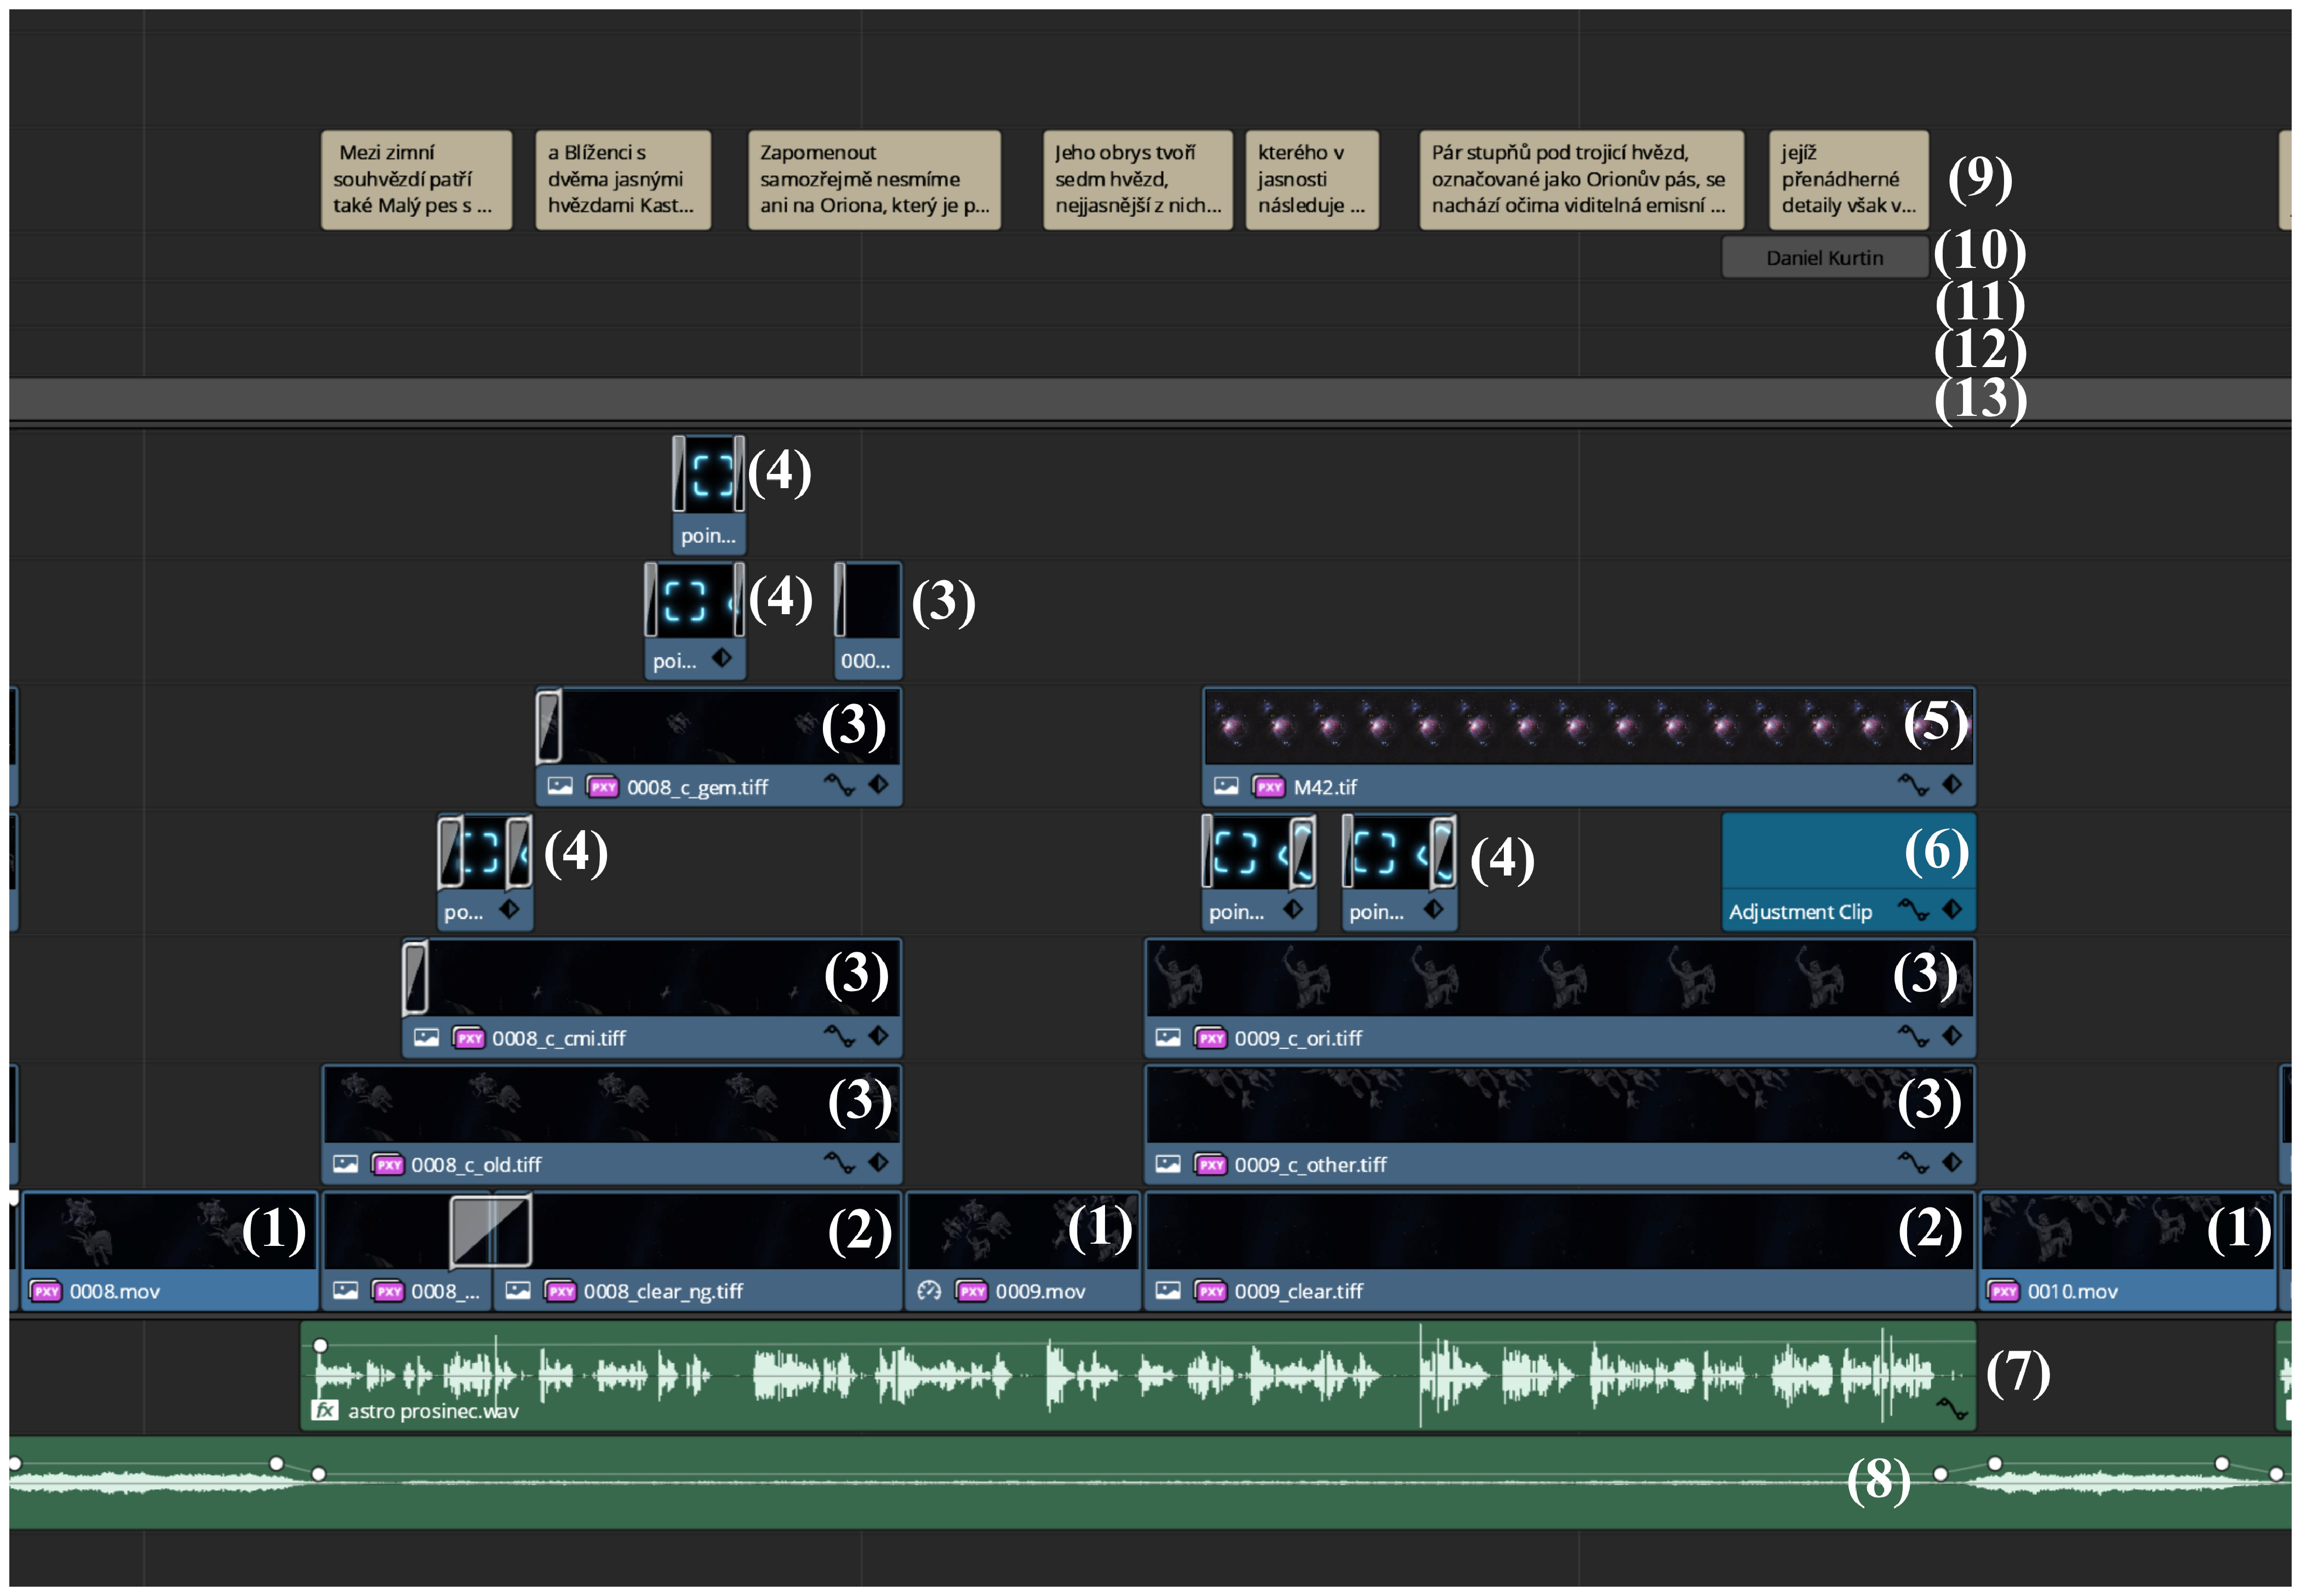
\includegraphics[width=1\textwidth]{timeline_annotated.eps}
\caption{Snímek jedné ze scén z finálního videa. Každá důležitá stopa má přiřazené číslo. Vysvětlení v oddílu \ref{makingof:resolve:merging}}
\label{img:timeline}
\end{figure}

\begin{figure}[ht]
\centering

\includegraphics[width=.5\textwidth]{pointer.eps}
\caption{Animace zvaná pointer, využívaná pro upřesnění pozice objektu, o kterém v daném momentě mluví scénář.}
\label{img:pointer}
\end{figure}

\begin{figure}[ht]
\centering
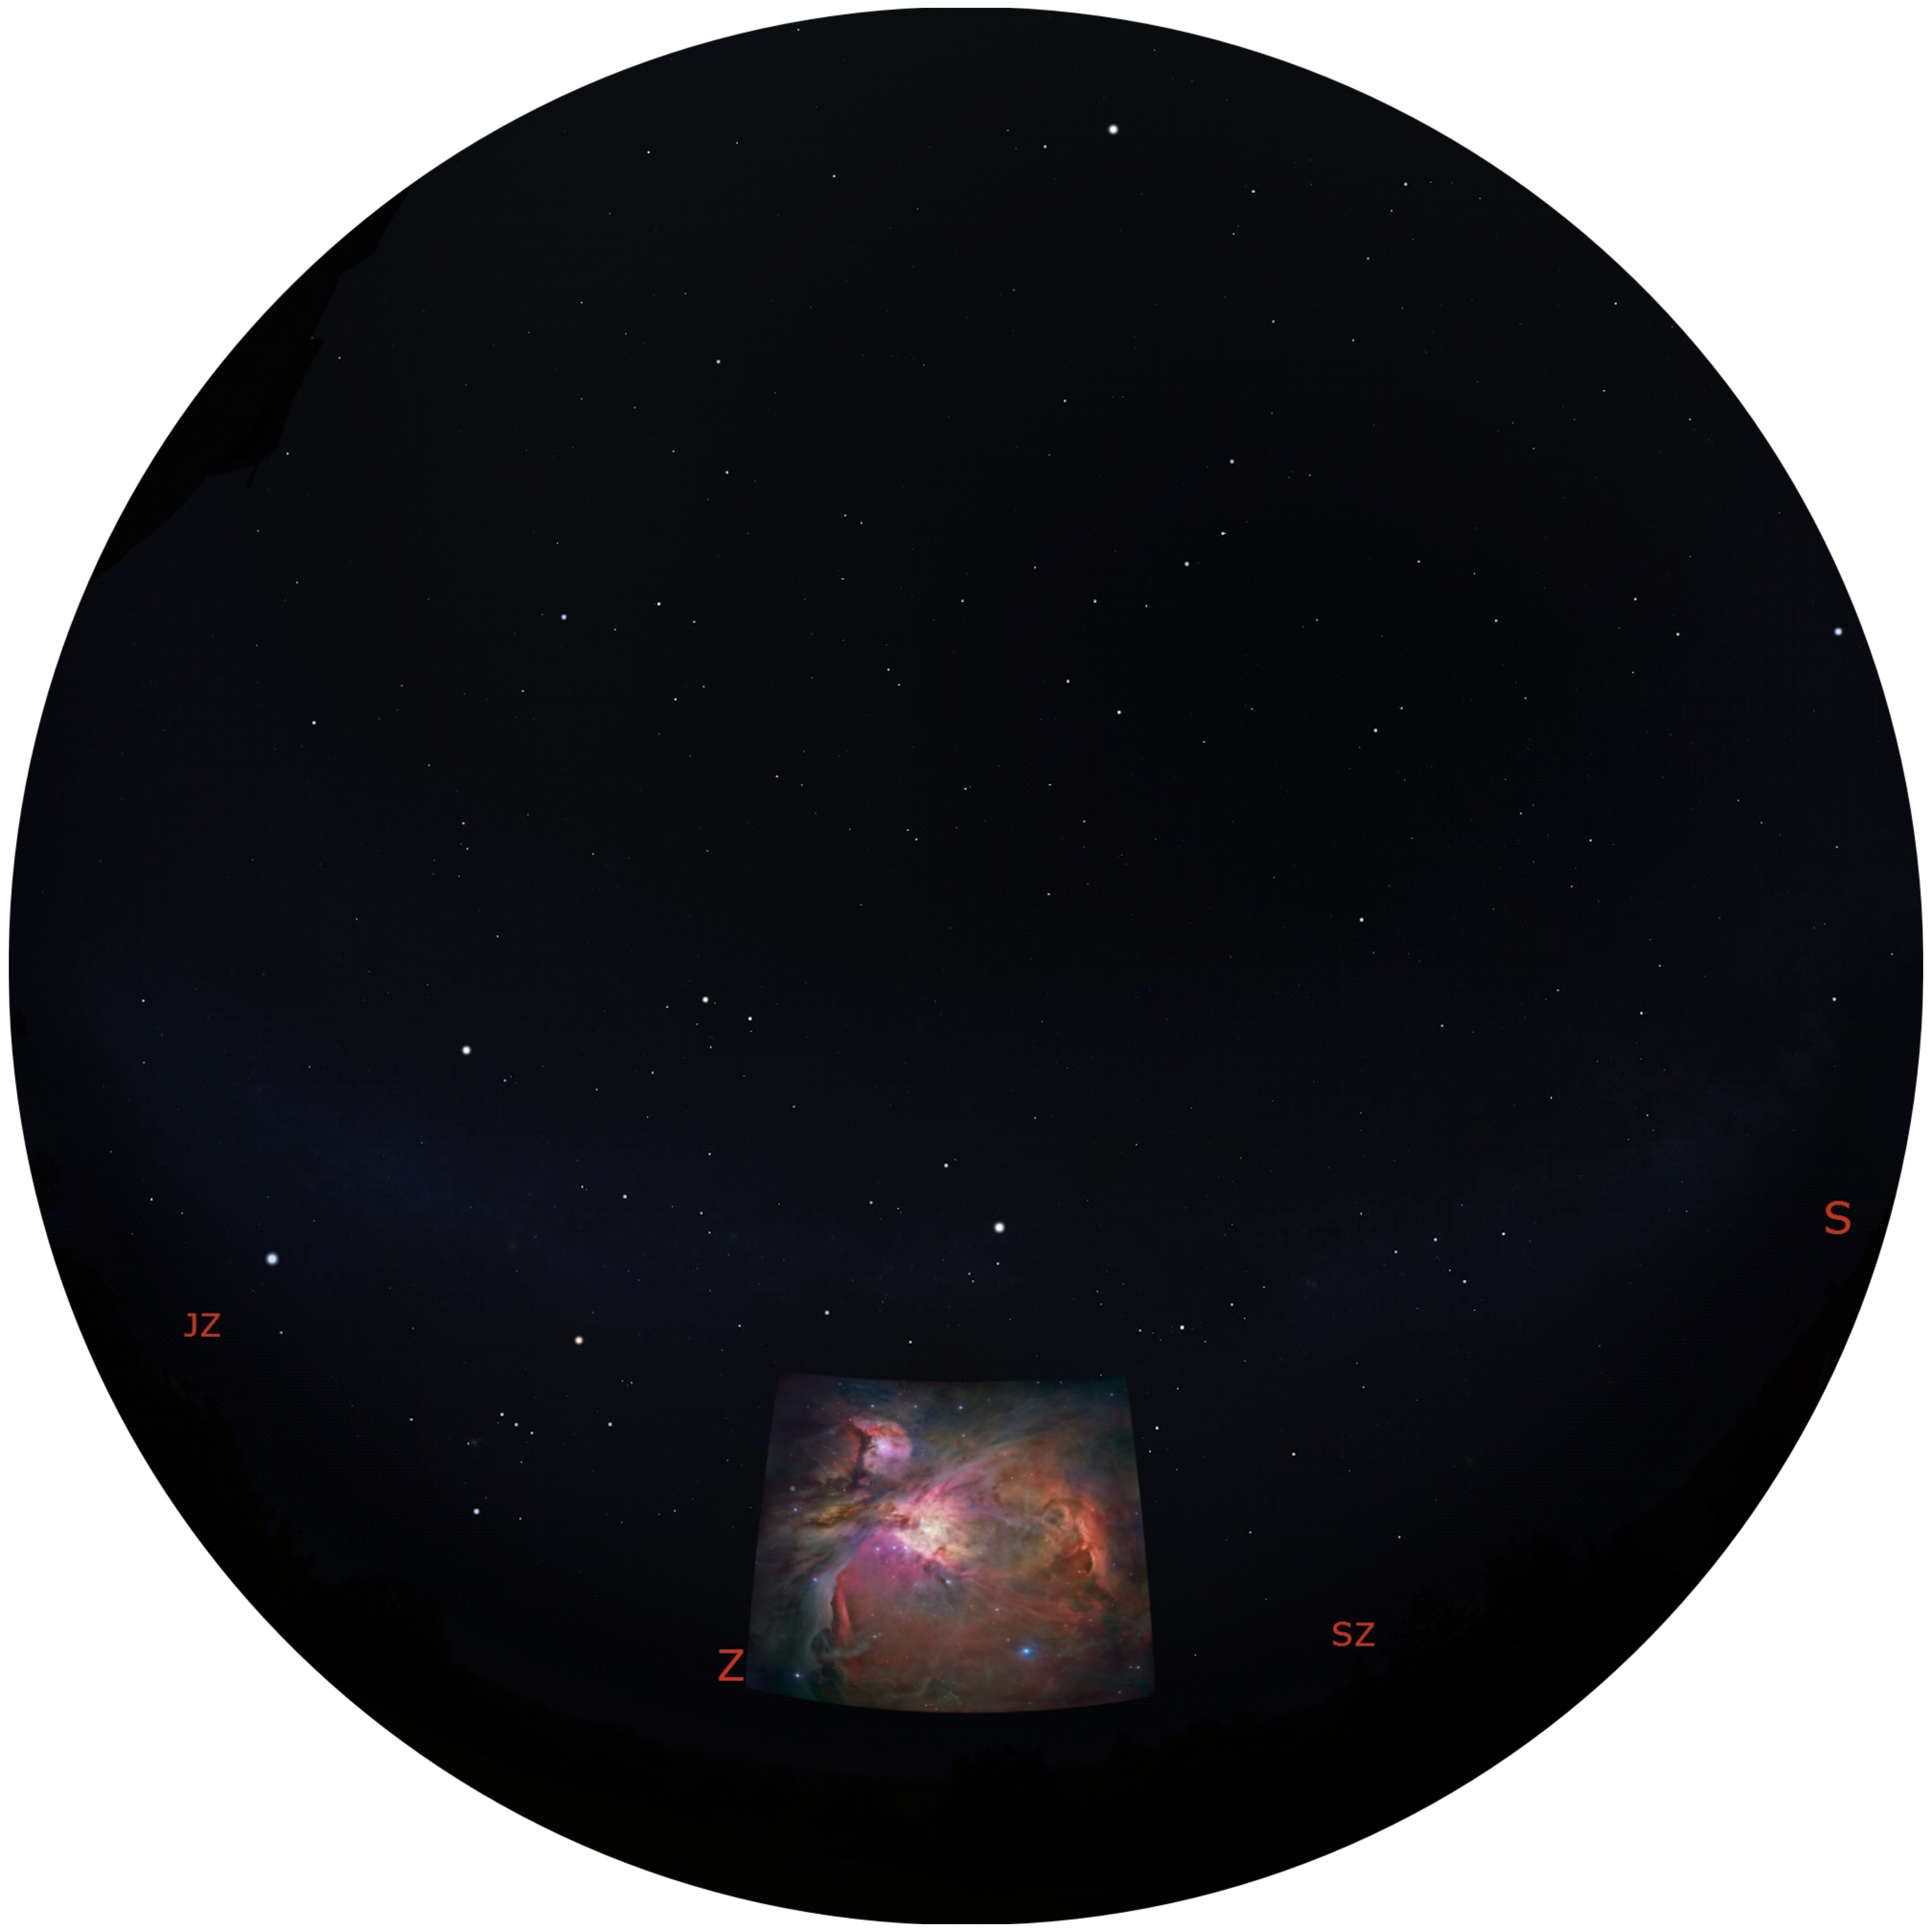
\includegraphics[width=.7\textwidth]{prosinec.eps}
\caption{Demonstrace našeho prvního videa.}
\label{img:prosinec}
\end{figure}

\begin{figure}[ht]
\centering
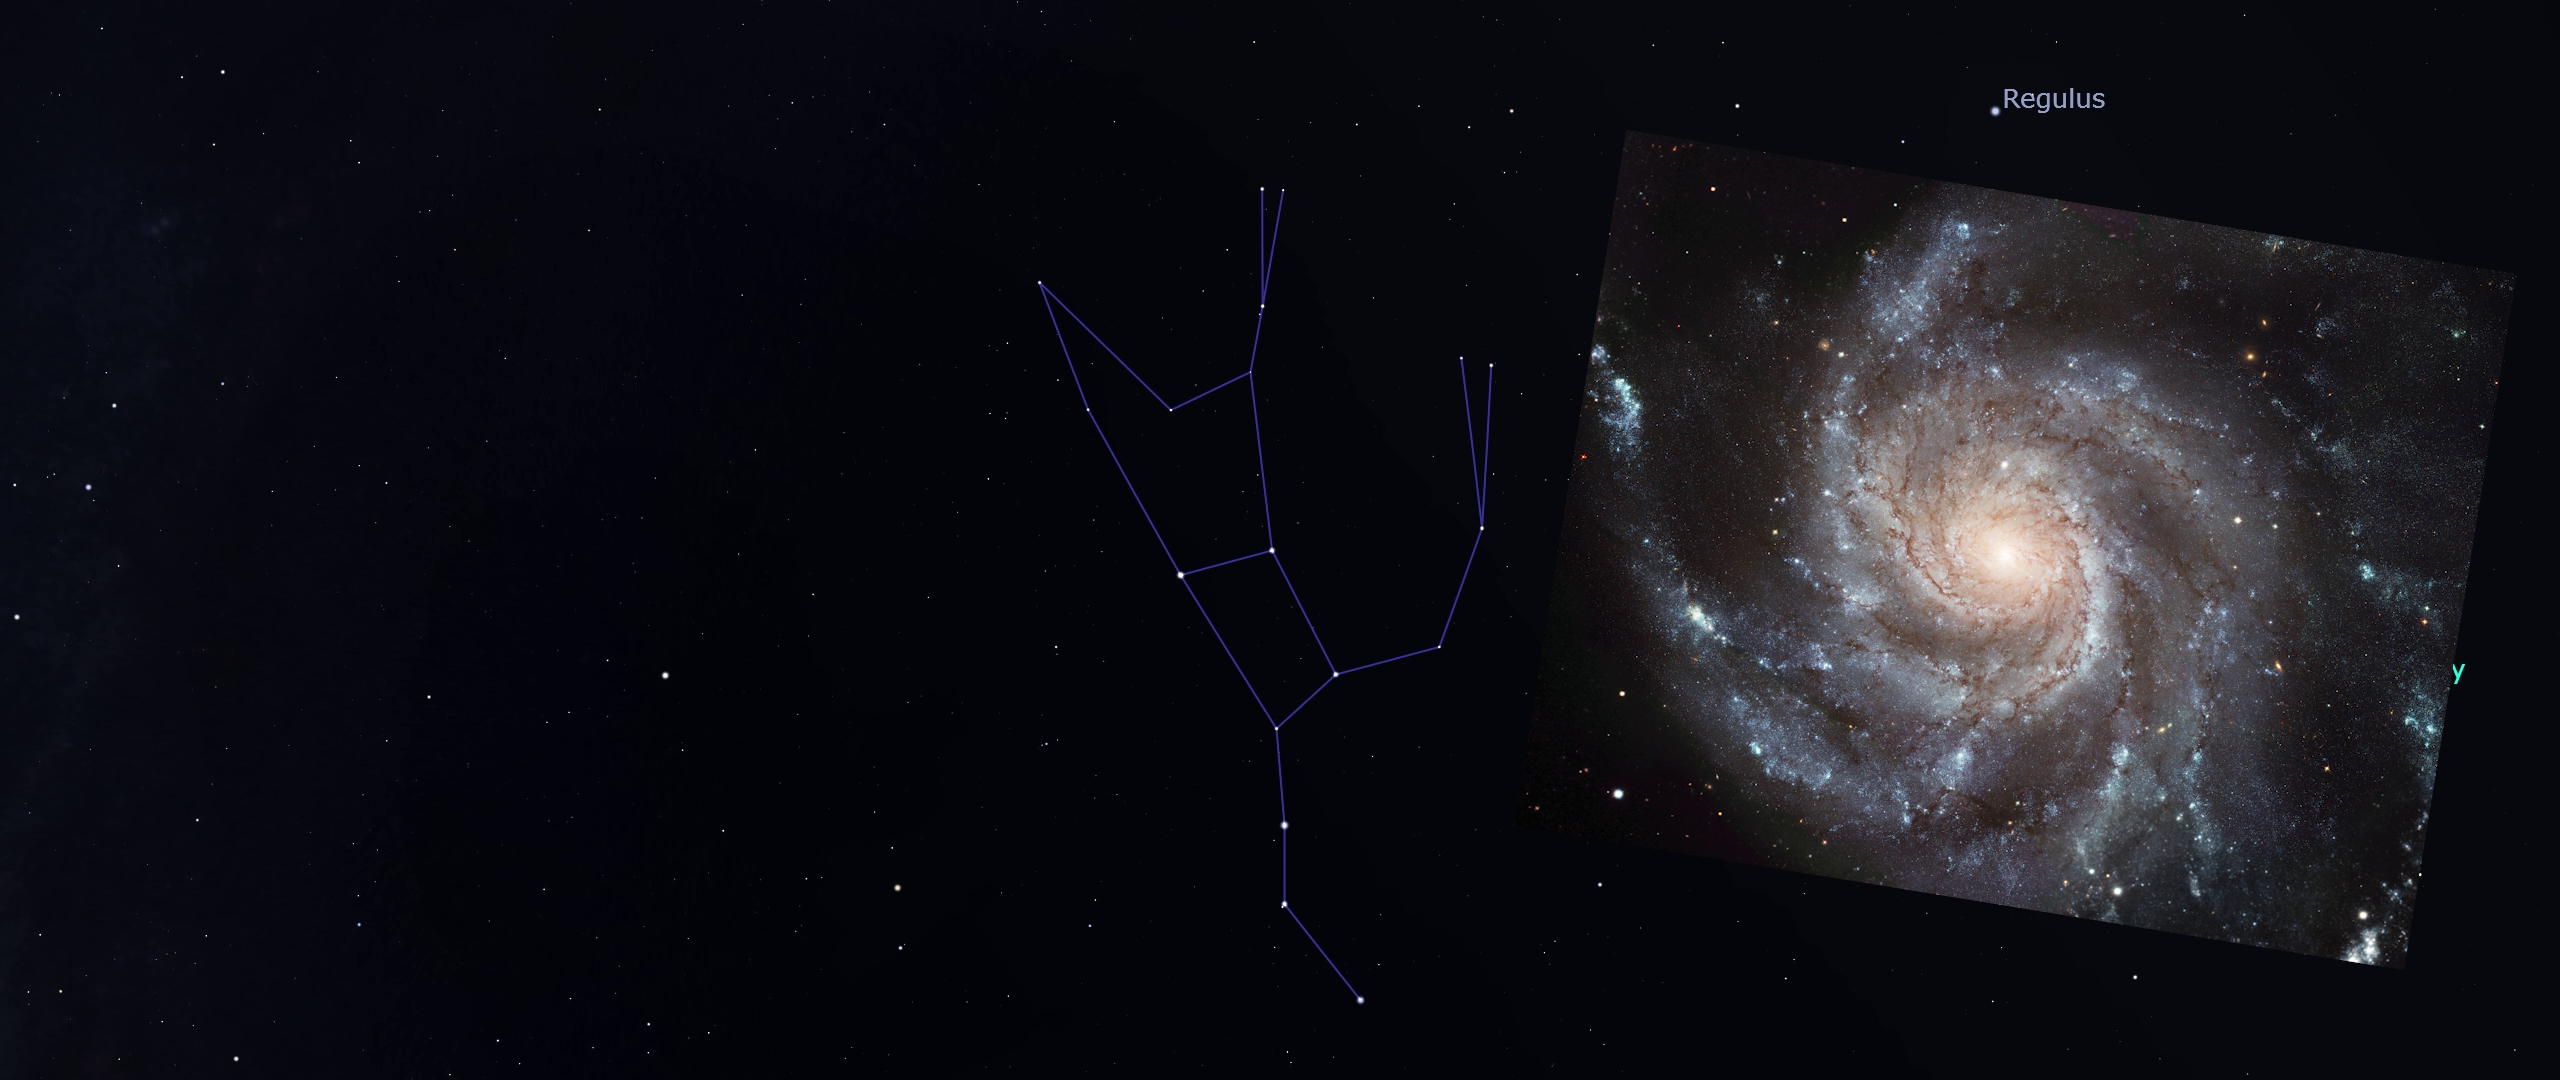
\includegraphics[width=.85\textwidth]{brezen.png}
\caption{Demonstrace našeho prvního videa.}
\label{img:brezen}
\end{figure}


\begin{figure}[ht]
\centering
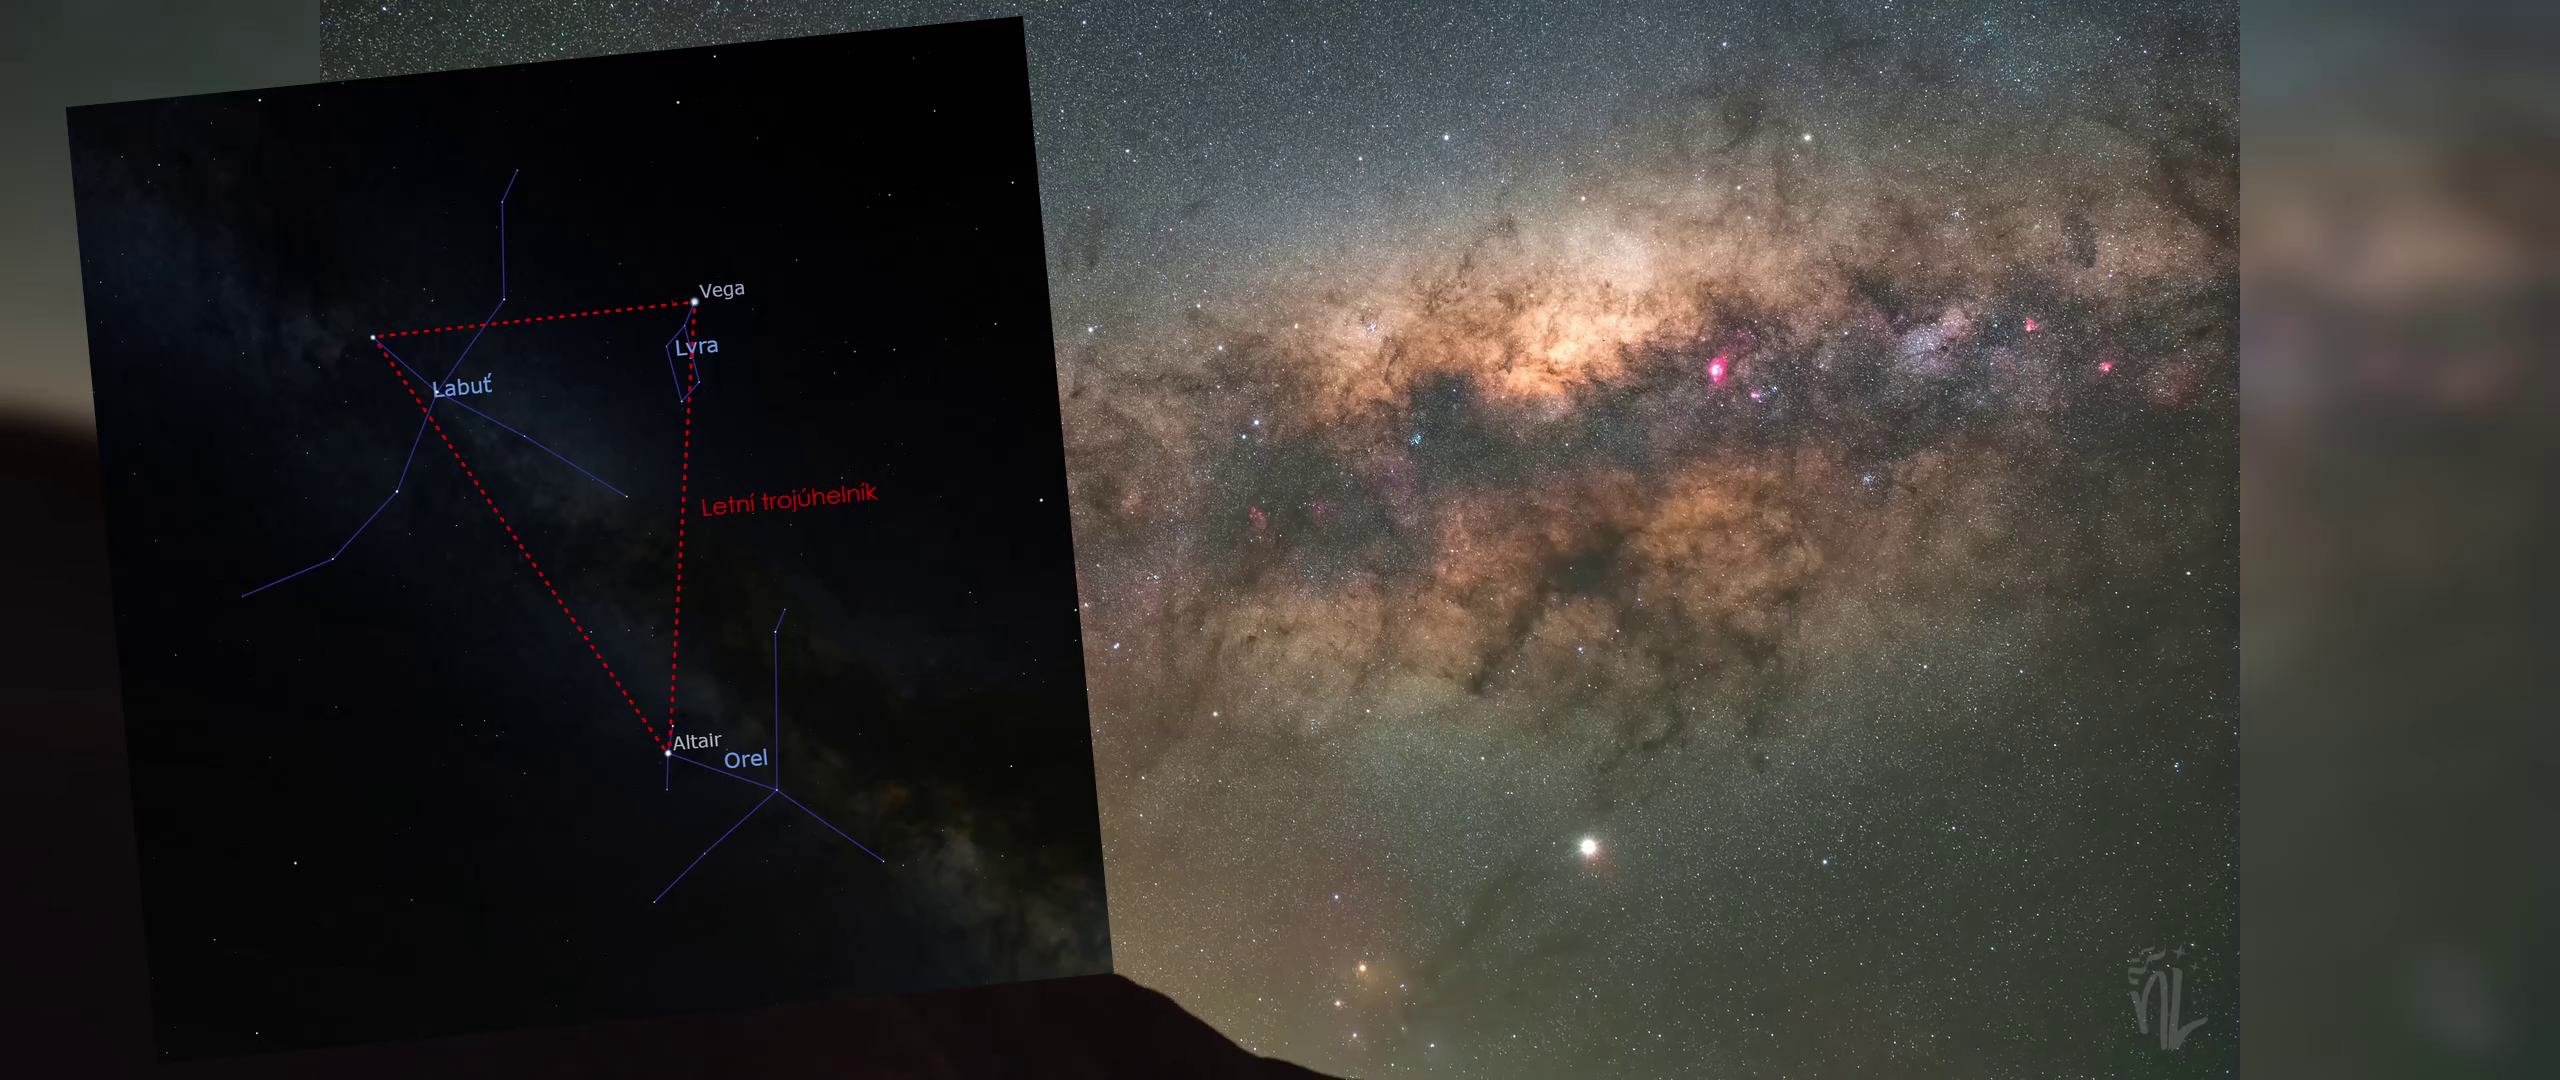
\includegraphics[width=.85\textwidth]{cervenec.png}
\caption{Demonstrace našeho prvního videa.}
\label{img:cervenec}
\end{figure}

\begin{figure}[ht]
\centering
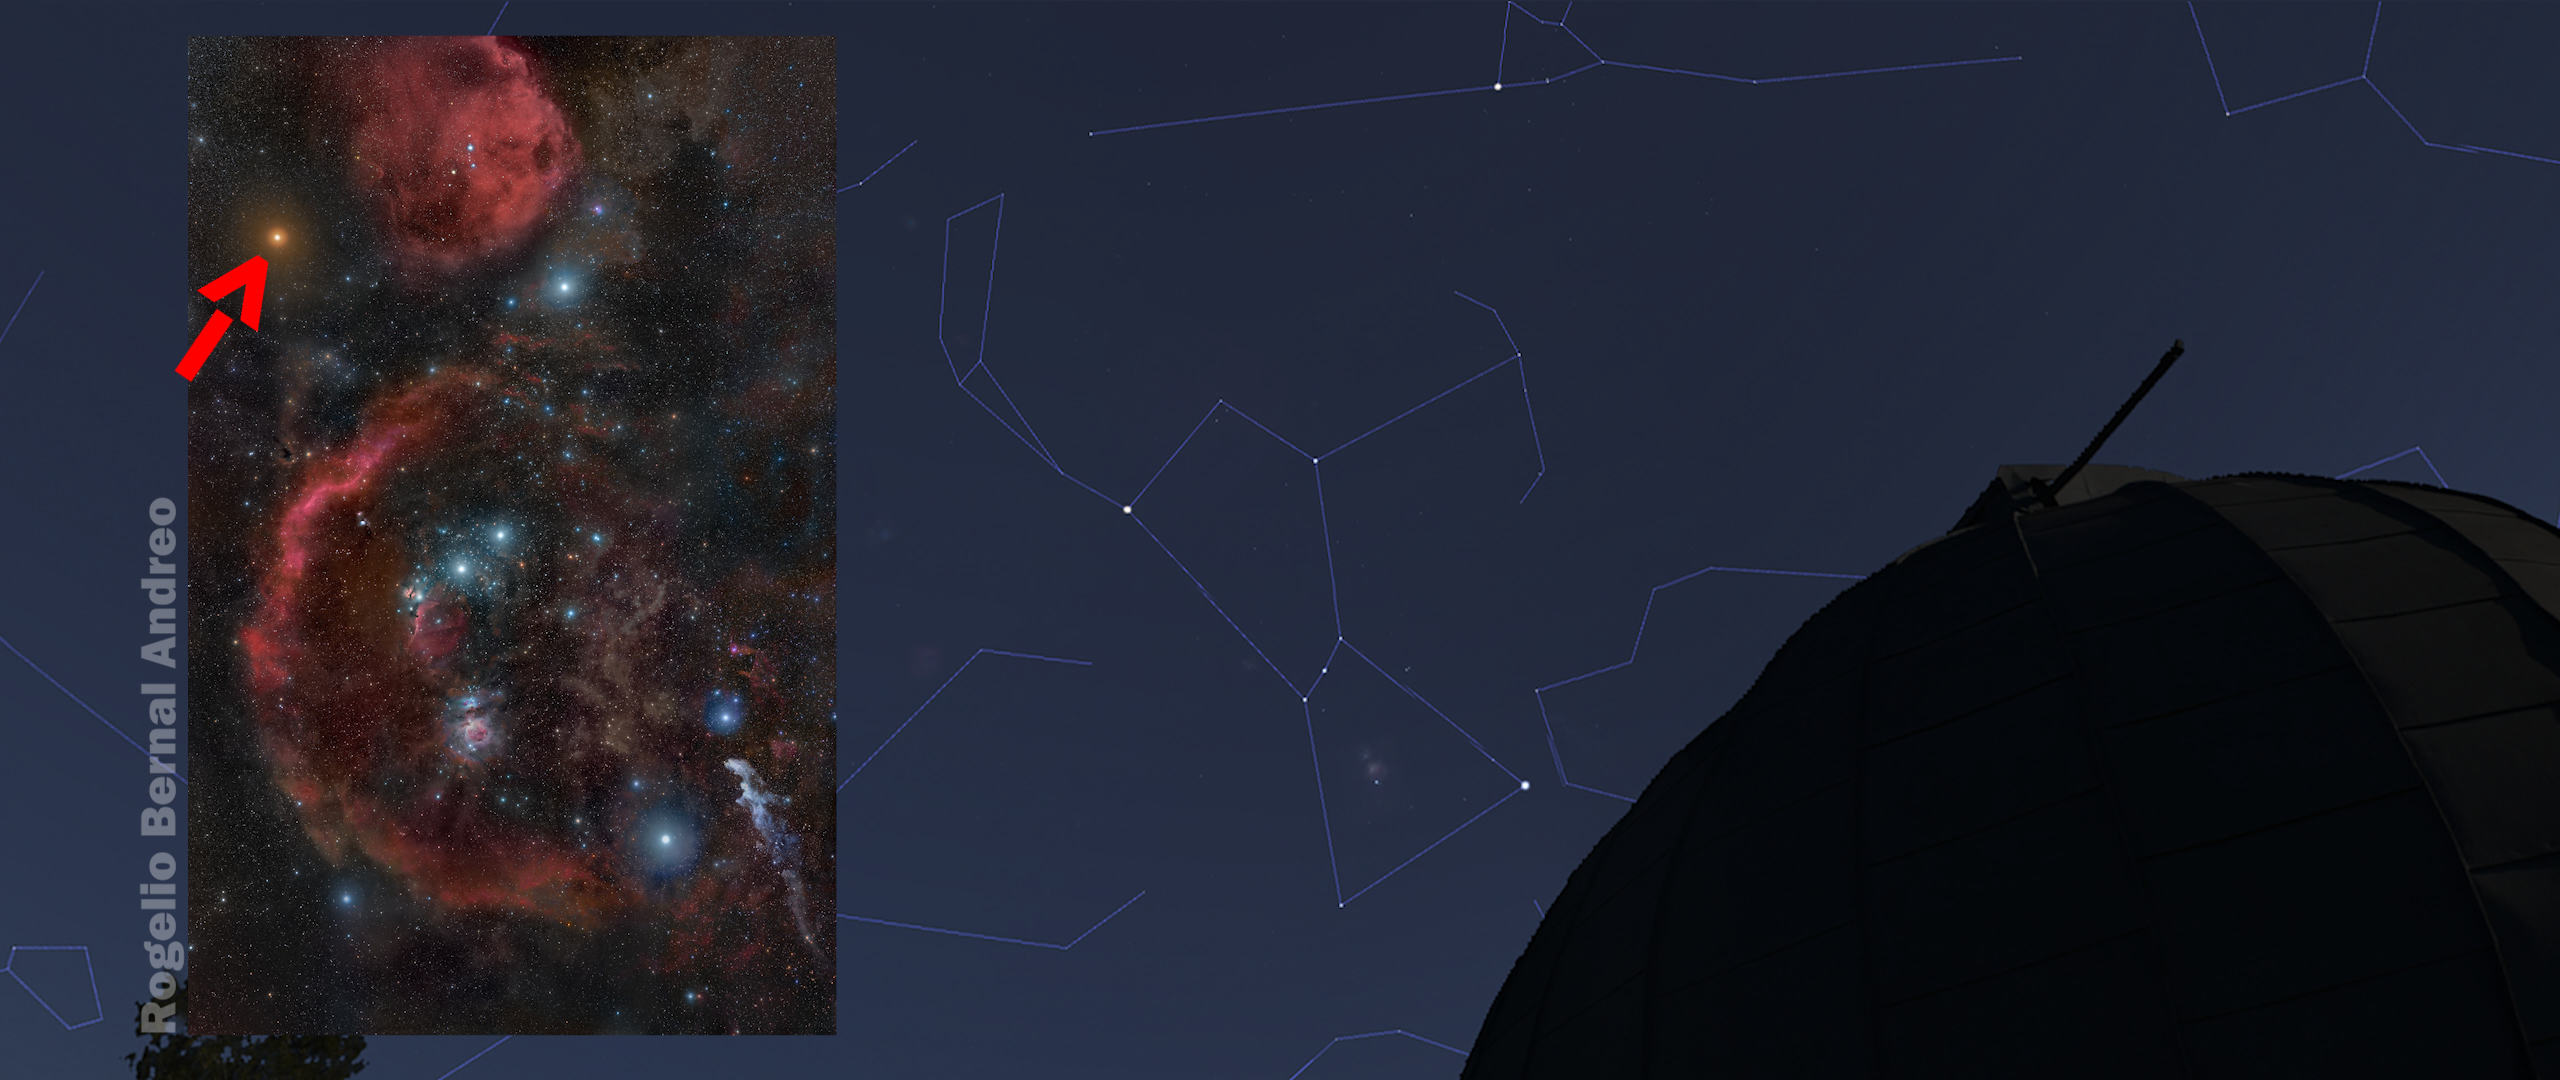
\includegraphics[width=.85\textwidth]{unor.png}
\caption{Demonstrace našeho prvního videa.}
\label{img:unor}
\end{figure}

\begin{figure}[ht]
	\begin{subfigure}{0.4\textwidth}
		\begin{tikzpicture}[scale=0.75]
			\begin{axis}
			[
			    xlabel={$t$}, 
			    ylabel={$x$}, 
			    xmin=0, 
			    xmax=1, 
			    ymin=0, 
			    ymax=1, 
			    axis lines=left
			]
				\addplot[no marks, solid, domain=0:1, samples=50] {x};
			\end{axis}
		\end{tikzpicture}
		\caption{Závislost $x$ na $t$ pro základní lineární interpolaci}
	\end{subfigure}\hfill
	\begin{subfigure}{0.4\textwidth}
		\begin{tikzpicture}[scale=0.75]
			\begin{axis}
			[
			    xlabel={$t$}, 
			    ylabel={$\frac{dx}{dt}$}, 
			    axis lines=left
			]
				\addplot[no marks, solid, domain=0:1, samples=50] {1};
			\end{axis}
		\end{tikzpicture}
		\caption{$\frac{dx}{dt}$ pro základní lineární interpolaci}
	\end{subfigure}
	\captionsetup{name=Graf}
	\caption{Graf znázorňující hodnotu a rychlost změny výstupu implementace lineární interpolace s kvadratickým přechodem}
	\label{graph:lerp_linear}
\end{figure}

\begin{figure}[ht]
	\begin{subfigure}{0.4\textwidth}
		\begin{tikzpicture}[scale=0.75]
			\begin{axis}
			[
			    xlabel={$t$}, 
			    ylabel={$x$}, 
			    xmin=0, 
			    xmax=1, 
			    ymin=0, 
			    ymax=1, 
			    axis lines=left
			]
				\addplot[no marks, solid, domain=0:1, samples=50] {3*pow(x,2) - 2*pow(x,3)};
			\end{axis}
		\end{tikzpicture}
		\caption{Závislost $x$ na $t$ pro základní lineární interpolaci}
	\end{subfigure}\hfill
	\begin{subfigure}{0.4\textwidth}
		\begin{tikzpicture}[scale=0.75]
			\begin{axis}
			[
			    xlabel={$t$}, 
			    ylabel={$\frac{dx}{dt}$}, 
			    axis lines=left
			]
				\addplot[no marks, solid, domain=0:1, samples=50] {6*x - 6*pow(x,2)};
			\end{axis}
		\end{tikzpicture}
		\caption{$\frac{dx}{dt}$ pro základní lineární interpolaci}
	\end{subfigure}
	\captionsetup{name=Graf}
	\caption{Graf znázorňující hodnotu a rychlost změny výstupu implementace lineární interpolace s kvadratickým přechodem}
	\label{graph:lerp_quadr}
\end{figure}
\end{document}
